\newpage
\chapter{Projektmanagement}
Anhand der oben beschriebenen Arbeitsphasen werden die folgenden vier Meilensteine definiert. Die Meilensteine markieren jeweils das Ende einer Projektphase und haben einen Fertigstellungstermin. Beim Erreichen eines Meilensteins wird die bisherige Arbeit bewertet und Beschlüsse über den weiteren Projektverlauf gefällt. Insgesamt dienen die Meilensteine dem Projektcontrolling.
\section{Meilensteine}
Es werden die folgenden vier Meilensteine definiert. Die Meilensteine
beinhalten   eine Sammlung von Aufgaben und haben einen
Fertigstellungstermin. Sie markieren das Ende einer Projektphase. Sie
werden für das Projektcontrolling verwendet. 
%\todo{fünf Meilensteine definieren}
	\begin{itemize}
		\item MS1: Theorie und Recherchephase abgeschlossen und zu 80\% dokumentiert, ein Anforderungsdokument wurde erstellt
		\item MS2: Zwischenpräsentation, Vorstellen der ersten vier Antennenkonzepte
		\item MS3: Design und Prototyping, Antennensystem simulieren, produzieren, messen und bewerten
		\item MS4: Engeenieringmodel ist gefertigt und dokumentiert
	\end{itemize}

\section{Projektsitzungen und Gesprächsnotizen}
Die Gesprächsnotizen dienen den Projektverlauf nachvollziehbar zu dokumentieren. Sie werden jeweils nach den Projektsitzungen mit dem Betreuer Prof. Marcel Joss angestellt. Die jeweiligen Arbeitspakete von der vergangenen Woche und der kommenden Woche werden an den Sitzungen besprochen und dokumentiert. Beschlüsse die für den Verlauf der BDA relevant sind werden besprochen und dokumentiert
\section{Vorgehensmodell}
mit Arbeitspaken und Zeitdauer der Arbeits Phasen
\begin{figure}[!ht]
	\begin{center}
		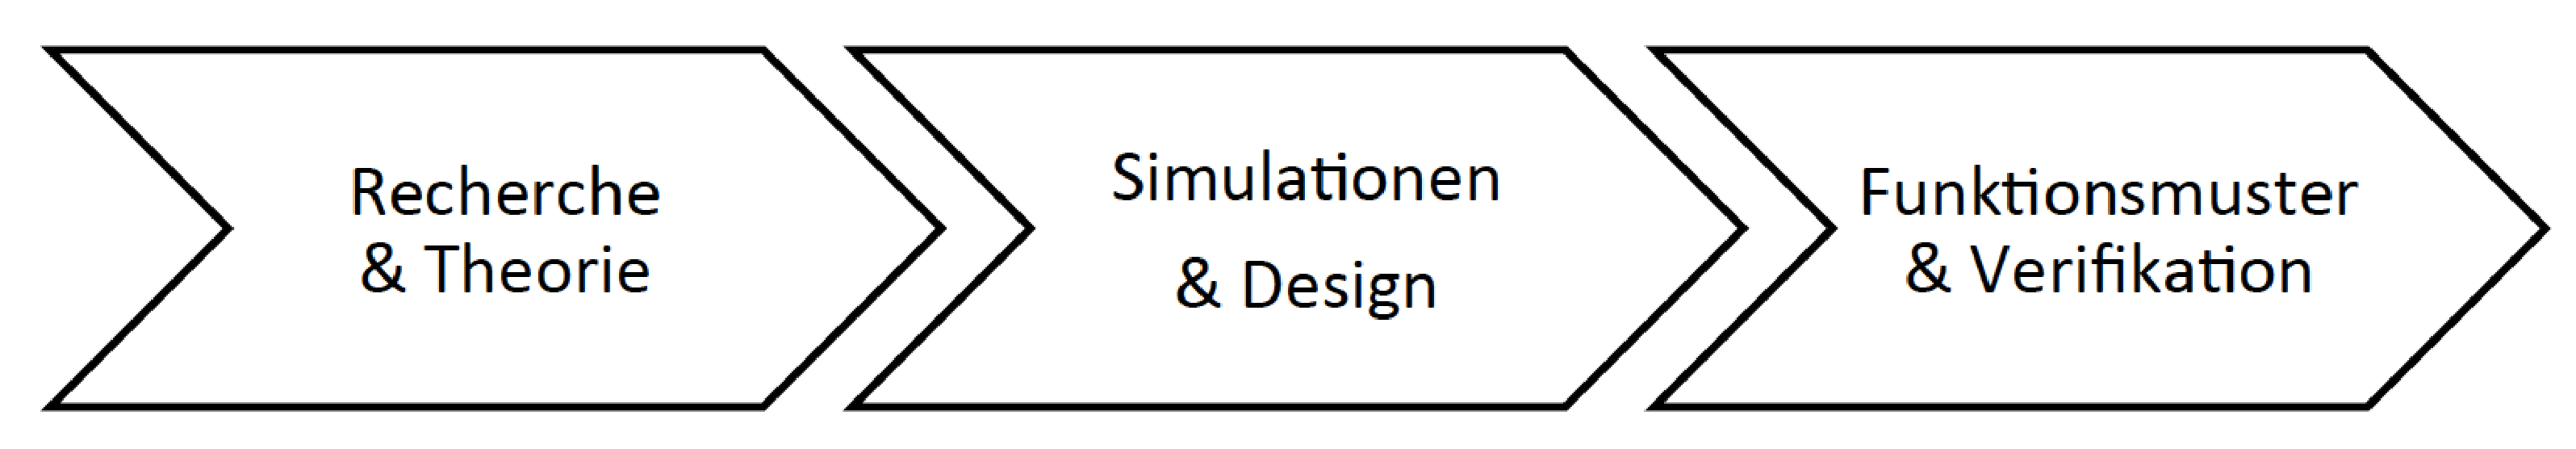
\includegraphics[width=11cm]{content/bilder/Vorgehensmodell.pdf}%
	\end{center}
	\caption{Vorgehensmodell}
	\label{Vorgehensmodell}
\end{figure}
\subsection{Arbeitspakete}
Welche Arbeitspacke und was beinhalten diese
\subsection{Ressourcenplanung}
Mann und Material 
\subsection{Zeitplan}
Welche Phasen wie lange
\subsection{Risikoanalyse}
zwei drei Riksiken
